%\documentclass[12pt,a4paper]{article}
\documentclass[10pt,journal,compsoc]{IEEEtran}
\usepackage[utf8]{inputenc}
\usepackage[english]{babel}
\usepackage{amsmath}
\usepackage{amsfonts}
\usepackage{amssymb}
\usepackage{graphicx}
\usepackage{algorithm,algorithmic}
\usepackage{xcolor}
%\documentclass[runningheads]{llncs}

\begin{document}

%\begin{center}
%\textbf{\LARGE Multi-core synthesis and maximum satisfiability applied to obtain optimal sizing of solar photovoltaic systems} \\
\title{Multi-core synthesis and maximum satisfiability applied to obtain optimal sizing of solar photovoltaic systems}
%\hfill \break
%IEEE Transactions on Computers \\
%
%Edilson Galvão, Alessandro Trindade, and Lucas Cordeiro \\
%\end{center}
\author{Edilson~Galvão, Alessandro~Trindade, and Lucas~Cordeiro% <-this % stops a space
\IEEEcompsocitemizethanks{
\IEEEcompsocthanksitem{E. Galvão is with MSc student in the Post-graduate Program in Electrical Engineering, Manaus, Brazil, e-mail: esj.galvao@gmail.com.}
\IEEEcompsocthanksitem{A. Trindade is with the Department of Electricity, Federal University of Amazonas, Manaus, Brazil, e-mail: alessandrotrindade@ufam.edu.br.}% <-this % stops a space
\IEEEcompsocthanksitem{L. Cordeiro is with School of Computer Science, The University of Manchester, UK, e-mail: lucas.cordeiro@manchester.ac.uk.}}% <-this % stops a space
}

% make the title area
\maketitle

% For peer review papers, you can put extra information on the cover
% page as needed:
% \ifCLASSOPTIONpeerreview
% \begin{center} \bfseries EDICS Category: 3-BBND \end{center}
% \fi
%
% For peerreview papers, this IEEEtran command inserts a page break and
% creates the second title. It will be ignored for other modes.
\IEEEpeerreviewmaketitle

%%%%%%%%%%%%%%%%%%%%%%%%%%%%%%%%%%%%%%%%%%%%%%%%%%%%%%%%
\section*{Sizing Stand-alone Solar PV Systems}
\label{sec:sizing}
%%%%%%%%%%%%%%%%%%%%%%%%%%%%%%%%%%%%%%%%%%%%%%%%%%%%%%%%

A PV system is illustrated in Fig.\ref{fig:blockdiagram}. It employs the PV generator (\textit{panel or an array}), which is a semiconductor device that can convert solar energy into DC electricity. For night hours or rainy days, we hold \textit{batteries}, where power can be stored and used. The use of batteries as a storage form implies the presence of a \textit{charge controller}~\cite{Hansen}. The PV arrays produce DC, and therefore when the PV system contains an AC load, a DC/AC conversion is required (\textit{inverter}). The \textit{AC load} dictates the behaviour of the AC electrical load from the house that will be fed by the system.

\begin{figure}[h]
\fbox{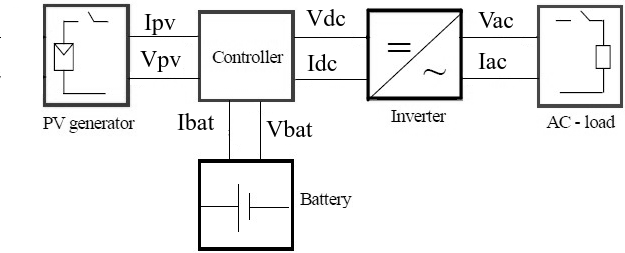
\includegraphics[width=0.45\textwidth]{blockdiagramPVS2_rev}}
\centering
\caption{Block diagram for a typical stand-alone PV system~\cite{Hansen}.}
\label{fig:blockdiagram} 
\end{figure}

The sizing check stage can ensure that the system meets the standard project steps related to the critical period method (worst month) for solar energy system sizing~\cite{Pinho} and adopting an MPPT (Maximum Power Point Tracking) charge controller, which is the most common in use. Firstly, we need to correct the daily energy consumption estimated for the load ($E_{consumption}$), which is carried out by Eq.~\eqref{eq:Ecorrected}, where the efficiency of batteries ($\eta_{b}$), controller ($\eta_{c}$), and inverter ($\eta_{i}$) are considered~\cite{Pinho}.

\begin{equation}
\label{eq:Ecorrected}
E_{corrected} = \dfrac{E_{consumption}}{\eta_{b} \times \eta_{c} \times \eta_{i} }
\end{equation}

We must estimate the total power that will be demanded from the PV panels, as defined by Eq. ~\eqref{eq:Pminpanel}. Where $Insolation$, also called solar irradiation or solar exposure, is expressed in terms of $kWh/m^{2}$ per day and depends on the site where the PV system will be deployed. \textcolor{black}{An empirical factor of $20$\% for losses is considered~\cite{Pinho}}, because $1.25 = 1 \mathbin{/} (1 - 0.2)$.

\begin{equation}
\label{eq:Pminpanel}
P_{min,panels} = \dfrac{1.25 \times E_{corrected}}{Insolation}
\end{equation}

On the one hand, the sizing must meet this requirement of minimum power supplied from the PV panels $P_{min,panels}$. On the other hand, the arrangement, if in series or parallel connections, it will depend on the charge controller specification of current $I_{c}$ and voltage $V_{c}$, as described by Eqs.~\eqref{eq:Icmin} and \eqref{eq:Vcmin}.

\begin{equation}
\label{eq:Icmin}
I_{c} \geq I_{total,PVpanels}
\end{equation}

\begin{equation}
\label{eq:Vcmin}
V_{c} \geq V_{total,PVpanels}
\end{equation}

Concerning the batteries, the energy $E_{b}$ to be demanded by the PV system, in order to meet the load requirements, is defined by Eq.~\eqref{eq:Ebat}.

\begin{equation}
\label{eq:Ebat}
E_{b} = \dfrac{Autonomy \times E_{corrected}}{DOD}
\end{equation}

\noindent Where $Autonomy$ is the number of days expected for the PV system to work even when rain or clouds avoid the recharging of batteries usually is a design definition and has a value ranging from $0.5$ to $2$ days. $DOD$ is the depth of discharge or the fraction of discharge. The $DOD$ is usually $25$\% for lead-acid batteries, and $80$\% for lithium batteries \textcolor{black}{and represent an intrinsic and empirical feature of those type of batteries~\cite{Pinho} in order to guarantee its lifetime}; that represents a State of Charge ($SOC$) of $75$\% and $20$\% respectively, because $SOC=1-DOD$. However, it is worth separating the $DOD$ into two different definitions when the battery autonomy is larger than one day ($24$ hours). \textcolor{black}{Therefore, the definition given here is for a maximum of $DOD$}. When we deal with daily $DOD$, we will call it $DOD_{day}$, and obviously, the sum of every $DOD_{day}$ can not exceed the maximum $DOD$.

In order to define the $DOD_{day}$, we use Eq.~\eqref{eq:DODday}. Moreover, the minimum current from the DC bus is defined by Eq.~\eqref{eq:Idcbus}. This equation is important to define the battery arrangement of the system (series and parallel connections). Where $V_{system}$ is the DC voltage of the bus.


\begin{equation}
\label{eq:DODday}
DOD_{day} = \dfrac{E_{corrected} \times 100}{E_{b}}
\end{equation}

\begin{equation}
\label{eq:Idcbus}
I_{min,DCbus} = \dfrac{E_{b}}{V_{system}}
\end{equation}

As for batteries, we must first define the total capacity of the battery bank, which can be described as shown in Eq.~\ref{eq:Cbank}. where $ E_{load} $ is the average energy consumed by the load corrected according to PV equipment efficiency, and $ \eta_{b} $ is the efficiency of the battery.

\begin{equation}
\label{eq:Cbank}
C_{bank} = \dfrac{Autonomy \times E_{load}}{DOD \times \eta_{b} \times V_{system}}
\end{equation}

Eq.~\ref{eq:batcheck} then performs the final sizing check, considering the number of batteries in series ($ N_{BS} $) and the number of batteries in parallel ($ N_{BP} $) adopted in the project.

\begin{equation}
\label{eq:batcheck}
\left( N_{BS} \times N_{BP} \right) \geq N_{B}total
\end{equation}

The charge controller must initially meet the voltage requirement of the PV system, as described by Eq.~\eqref{eq:vcvsystem}.
 
\begin{equation}
\label{eq:vcvsystem}
V_{c} = V_{system}
\end{equation}

\textcolor{black}{The short circuit reference information ($I_{sc,ref}$) from the manufacturer's solar panel must be corrected because field temperature ($T$) is higher than nominal or laboratory temperature ($25^{\circ}C$), and the PV system is temperature dependent (heat can reduce output efficiency by 10-25\%), as described by Eq.~\eqref{eq:iscamb} for the ambient short-circuit current from the PV panel. $G$ is the solar irradiance from the deployment site, and $G_{ref}$ is defined as $1000$ $W/m^{2}$ by the manufacturers.}

\begin{equation}
\label{eq:iscamb}
I_{sc,amb} = \dfrac{G}{G_{ref}} \left[ I_{sc,ref} + \mu_{I} \times (T-25) \right] 
\end{equation}

The controller must meet the maximum current from the PV array given by Eqs.~\eqref{eq:icmin} and~\eqref{eq:icicmin}. Where $N_{PP}$ is the number of parallel panels adopted.

\begin{equation}
\label{eq:icmin}
I_{c,min} = I_{sc,amb} \times N_{PP}
\end{equation}

\begin{equation}
\label{eq:icicmin}
I_{c} \geq I_{c,min}
\end{equation}

The number of controllers required for the off-grid PV system, as defined by \cite{Yatimi}, is calculated using Eq.~\eqref{eq:numberofcmin}. Besides, the final sizing check is performed by Eq.~\eqref{eq:numberofc}, which validates the number of controllers adopted.

\begin{equation}
\label{eq:numberofcmin}
\begin{split}
number_{controllers} = \dfrac{Total \, max \, power \, of \, PV}{Controller \, max \, power} \\ = \dfrac{P_{m,ref} \times N_{TP}}{V_{system} \times I_{controller,max}}
\end{split}
\end{equation}

\begin{equation}
\label{eq:numberofc}
N_{controller} \geq number_{controllers}
\end{equation}

The inverter sizing check is performed through three equations. Eq.~\eqref{eq:vindc} ensures that the input voltage of the controller meets the system voltage. Eq.~\eqref{eq:voutac} ensures that the output voltage of the controller meets the AC voltage of the load, i.e., the outlet voltage. Finally, Eq.~\eqref{eq:invcheck} ensures that the controller can support the total demand of the load ($Demand$) and the surge power ($P_{surge}$), where $V_{in}DC$ is the nominal input voltage, and $V_{out}AC$ is the nominal output voltage of the inverter; $MAX_{AC,ref}$ is the peak power that the inverter can support.

\begin{equation}
\label{eq:vindc} 
V_{in}DC = V_{system}
\end{equation}

\begin{equation}
\label{eq:voutac} 
V_{out}AC = V_{AC}
\end{equation}

\begin{equation}
\label{eq:invcheck} 
\left[ (Demand \leq P_{AC,ref}) \, and \, (P_{surge} \leq MAX_{AC,ref}) \right]
\end{equation}

Some inverter models allow parallel operation of more than one unit, besides the integration to create bi- and three-phase circuits. It is advisable to use pure sine wave inverters for electronic loads sensitive to harmonic distortion waves.

Besides that, it is crucial to verify the compatibility between the charge controller and inverter because some models are not compatible with equipment from other manufacturers. Furthermore, it is vital to select an inverter power that is lower than (or equal) the charge controller power, because the demand from the electric load causes the inverter to transfer this demand from the DC side. Then the controller can be overcharged during this operation and burn.

\bibliographystyle{IEEEtran}
\bibliography{references}


\end{document}
